\chapter{Transformers for Segmentation: From DETR to Mask2Former}\label{ch:transformers}

\section{Introduction}\label{sec:tr-intro}
In this chapter we build up the architecture of the final model one idea at a time. We assume that
the reader knows convolutional networks, but not that they remember the details of transformers, so
we start from the attention operation itself (Section~\ref{sec:tr-attention}). We then describe how
vision transformers, and in particular the Swin Transformer, adapt attention to images
(Section~\ref{sec:tr-swin}). Section~\ref{sec:tr-detr} introduces DETR, which treats detection as the
prediction of a set, and Section~\ref{sec:tr-maskformer} introduces MaskFormer, which extends this
idea from boxes to masks. Section~\ref{sec:tr-m2f} describes Mask2Former, the model we used, in
detail, including its loss and the way its outputs are turned into scored masks. Finally,
Section~\ref{sec:tr-why} explains why this architecture suits filaments.

\section{Attention}\label{sec:tr-attention}
A transformer operates on a \emph{set} of $n$ vectors called \keyterm{tokens},
$\mathbf{x}_1,\dots,\mathbf{x}_n\in\R^d$. In an image model, a token usually stands for a small patch
of pixels. The central operation, \keyterm{attention}~\citep{attention}, lets every token gather information from every
other token, weighted by how relevant each one is. Each token is projected in three ways by learned
matrices:
\begin{equation}
\mathbf{q}_i = W_Q\mathbf{x}_i, \qquad \mathbf{k}_j = W_K\mathbf{x}_j, \qquad \mathbf{v}_j = W_V\mathbf{x}_j .
\end{equation}
The \keyterm{query} $\mathbf{q}_i$ describes what token $i$ is looking for, the \keyterm{key}
$\mathbf{k}_j$ describes what token $j$ offers, and the \keyterm{value} $\mathbf{v}_j$ is what token
$j$ passes on if it is chosen. The output for token $i$ is a weighted mean of all the values, with
weights given by a softmax over the similarities between its query and every key:
\begin{equation}
\mathbf{y}_i = \sum_{j=1}^{n} a_{ij}\,\mathbf{v}_j, \qquad
a_{ij} = \frac{\exp(\mathbf{q}_i^{\top}\mathbf{k}_j/\sqrt{d_k})}{\sum_{j'}\exp(\mathbf{q}_i^{\top}\mathbf{k}_{j'}/\sqrt{d_k})}.
\end{equation}
Stacking the vectors as the rows of matrices gives the familiar form
\begin{equation}
\operatorname{Attention}(Q,K,V) = \softmax\!\Big(\frac{QK^{\top}}{\sqrt{d_k}}\Big)V,
\label{eq:tr-attention}
\end{equation}
where the softmax is taken along each row (Figure~\ref{fig:tr-attention}). The factor $1/\sqrt{d_k}$
matters. If the components of $\mathbf{q}$ and $\mathbf{k}$ are independent with unit variance, their
dot product has variance $d_k$, and without the scaling, large dot products would push the softmax
into saturation, where its gradients vanish (Exercise~\ref{ex:tr-sqrt}).

\begin{figure}[t]
\centering
\begin{tikzpicture}[
  tok/.style={circle, draw=vizblue!80!black, fill=vizblue!15, minimum size=0.42cm, inner sep=0pt,
              font=\sffamily\scriptsize},
  wcell/.style={minimum size=0.42cm, inner sep=0pt, draw=white, line width=0.5pt}]
  \foreach \i in {1,...,5} \node[tok] (x\i) at (0,-\i*0.5) {$x_{\i}$};
  \foreach \row [count=\rw] in {{55,20,10,10,5},{15,50,20,10,5},{5,15,45,25,10},{5,10,25,45,15},{5,5,10,20,60}}{
    \foreach \wt [count=\col] in \row {
      \pgfmathtruncatemacro{\shade}{min(100,\wt*1.6)}
      \node[wcell, fill=vizblue!\shade!white] at (1.5+\col*0.42, -\rw*0.5) {};
    }
  }
  \foreach \i in {1,...,5} \node[tok, draw=vizorange!80!black, fill=vizorange!15] (y\i) at (5.0,-\i*0.5) {$y_{\i}$};
  \draw[flow] (0.35,-1.5) -- (1.62,-1.5);
  \draw[flow] (3.95,-1.5) -- (4.6,-1.5);
  \node[note] at (2.76,-0.02) {keys $j$ (who is asked)};
  \node[note, anchor=west, text width=4.4cm, align=left] at (5.6,-1.5)
       {row $i$: weights $a_{ij}$, summing to one; output $y_i=\sum_j a_{ij}v_j$};
  \node[note] at (2.76,-3.05) {query $i$ asks each key; darker means more weight};
\end{tikzpicture}
\caption{Self-attention on five tokens. Each row of the weight matrix is one token's softmax over all
the tokens, and its output is the corresponding weighted mean of their values.
\drawnin{book/chapters/ch11\_transformers.tex}}
\label{fig:tr-attention}
\end{figure}

Listing~\ref{lst:tr-attention} implements Equation~\eqref{eq:tr-attention} in a few lines, with an
optional mask of forbidden pairs that we will need in Section~\ref{sec:tr-masked}.

\begin{lstlisting}[caption={Scaled dot-product attention with an optional mask.},label=lst:tr-attention]
def attention(q, k, v, forbidden=None):         # q: (n, d); k and v: (m, d)
    scores = q @ k.T / math.sqrt(q.shape[-1])   # (n, m): how much each query wants each key
    if forbidden is not None:                   # boolean (n, m): pairs that may not attend
        scores = scores.masked_fill(forbidden, float("-inf"))   # exp(-inf) = 0 weight
    return scores.softmax(dim=-1) @ v           # each output: a weighted mean of the values
\end{lstlisting}

Three refinements complete the basic picture. First, \keyterm{multi-head attention} runs $h$
attention operations in parallel, on separate projections of dimension $d/h$, and concatenates the
results, so that different heads can attend to different things. Second, in \keyterm{self-attention}
the queries, keys and values all come from the same set of tokens, whereas in
\keyterm{cross-attention} the queries come from one set and the keys and values from another.
Mask2Former uses both: its object queries attend to each other, and they attend to the image.
Third, a transformer layer wraps attention and a small two-layer perceptron (MLP) in residual
connections and normalisation, computing $\mathbf{y} = \mathbf{x} + \operatorname{Attn}(\mathbf{x})$
and then $\mathbf{z} = \mathbf{y} + \operatorname{MLP}(\mathbf{y})$, with a layer
normalisation~\citep{ba2016} before or after each step.

\subsection{The cost of attention, and where positions come from}\label{sec:tr-positions}
The matrix $QK^{\top}$ has $n^2$ entries, so the time and memory that attention needs grow with the
\emph{square} of the number of tokens. A $2048\times2048$ photograph at stride 4 has $512^2 = 262{,}144$
tokens, and a full attention matrix over them would have about $7\times10^{10}$ entries. This single
fact shapes every design in the rest of the chapter.

Attention is also blind to the order of the tokens: permuting the tokens permutes the outputs and
changes nothing else. Information about position must therefore be added explicitly. The DETR family
of models~\citep{detr} adds a fixed \keyterm{sine positional embedding}, adapted from the original
transformer~\citep{attention}. For a feature map of width $W$ and a
column $j$, the normalised position is $\tilde x = 2\pi\,(j+\tfrac12)/W$, and the embedding
interleaves
\begin{equation}
\mathrm{PE}_{2i}(\tilde x) = \sin\!\big(\tilde x / T^{2i/D}\big), \qquad
\mathrm{PE}_{2i+1}(\tilde x) = \cos\!\big(\tilde x / T^{2i/D}\big), \qquad T = 10{,}000,
\label{eq:tr-sine}
\end{equation}
for $i=0,1,\dots,D/2-1$, with the same construction for the rows. Note the normalisation by $W$.
Positions are expressed as fractions of the extent of the input, so two pixels a fixed distance apart
receive embeddings that differ \emph{less} in a large input than in a small one.
Section~\ref{sec:train-sampling} shows why this detail forced us to train the final model on whole
photographs as well as on crops.

\section{Vision transformers and Swin}\label{sec:tr-swin}
The \keyterm{Vision Transformer} (ViT)~\citep{vit} cuts an image into patches of $16\times16$ pixels,
embeds each patch as a token, and applies global self-attention. At $224\times224$ pixels this gives
only 196 tokens, and ViT classifies images well. For segmentation at the native resolution of our
photographs, however, it fails on both of the counts above: the number of tokens explodes, and a
single feature map at stride 16 is far too coarse for a filament four pixels wide.

The \keyterm{Swin Transformer}~\citep{swin} makes attention local and hierarchical, like a
convolutional network. It does so with five ideas.
\begin{itemize}[leftmargin=*,itemsep=2pt]
\item \textbf{Small patches.} The tokens are patches of $4\times4$ pixels, so the first feature map
has stride 4.
\item \textbf{Windows.} Self-attention runs only within non-overlapping windows of $M\times M$ tokens,
with $M=7$. For a map of $h\times w$ tokens with $C$ channels, this reduces the cost of a layer from
$4hwC^2 + 2(hw)^2C$ for global attention to
\begin{equation}
\Omega_{\text{window}} = 4hwC^2 + 2M^2hwC,
\end{equation}
which is linear in the number of tokens.
\item \textbf{Shifted windows.} Alternate layers shift the grid of windows by $\lfloor M/2\rfloor$
tokens (Figure~\ref{fig:tr-swin}), so that information crosses the borders of the windows from one
layer to the next.
\item \textbf{Merging.} Between stages, each $2\times2$ group of tokens is concatenated and projected
to a single token, which halves the resolution and doubles the number of channels. The four stages
therefore produce feature maps at strides 4, 8, 16 and 32, which is the pyramid that a segmentation
head needs.
\item \textbf{Relative position.} Inside a window, a learned bias $B$ that depends only on the offset
between two tokens is added to the attention scores~\citep{shaw2018}, giving $\softmax(QK^{\top}/\sqrt{d_k} + B)\,V$.
\end{itemize}

\begin{figure}[t]
\centering
\begin{tikzpicture}[scale=0.34]
  % regular windows: 2 x 2 windows of 4 x 4 patches
  \fill[vizblue!18] (0,4) rectangle (4,8); \fill[vizorange!18] (4,4) rectangle (8,8);
  \fill[vizaqua!18] (0,0) rectangle (4,4); \fill[vizyellow!22] (4,0) rectangle (8,4);
  \draw[gridline, line width=0.3pt] (0,0) grid (8,8);
  \draw[inkprimary, line width=0.9pt] (0,0) rectangle (8,8) (4,0) -- (4,8) (0,4) -- (8,4);
  % shifted windows: borders at 2 and 6
  \begin{scope}[shift={(12,0)}]
    \fill[vizblue!18] (2,2) rectangle (6,6);
    \fill[vizorange!18] (6,2) rectangle (8,6); \fill[vizorange!18] (0,2) rectangle (2,6);
    \fill[vizaqua!18] (2,6) rectangle (6,8); \fill[vizaqua!18] (2,0) rectangle (6,2);
    \fill[vizyellow!22] (0,0) rectangle (2,2); \fill[vizyellow!22] (6,6) rectangle (8,8);
    \fill[vizyellow!22] (0,6) rectangle (2,8); \fill[vizyellow!22] (6,0) rectangle (8,2);
    \draw[gridline, line width=0.3pt] (0,0) grid (8,8);
    \draw[inkprimary, line width=0.9pt] (0,0) rectangle (8,8) (2,0) -- (2,8) (6,0) -- (6,8)
         (0,2) -- (8,2) (0,6) -- (8,6);
  \end{scope}
  \node[note] at (4,-1.6) {layer $\ell$: regular windows};
  \node[note] at (16,-1.6) {layer $\ell+1$: shifted by half a window};
\end{tikzpicture}
\caption{Swin's shifted windows on an $8\times8$ map of tokens, with windows of $4\times4$ tokens.
Attention runs only inside each window with a thick border. In the next layer the grid is shifted, so
tokens that were separated by a border now share a window. Pieces of the same colour on the right are
joined into one window by a cyclic shift of the map. \drawnin{book/chapters/ch11\_transformers.tex}}
\label{fig:tr-swin}
\end{figure}

The backbone of the final model is \keyterm{Swin-S} (``small''), which has 96 channels in its first
stage, 2, 2, 18 and 2 blocks in its four stages, with 3, 6, 12 and 24 attention heads respectively,
and windows of $7\times7$ tokens. It came pretrained as part of a complete Mask2Former that had been
trained on the COCO instance segmentation task.

\section{DETR: detection as set prediction}\label{sec:tr-detr}
Most detectors, including the YOLO models of Chapter~\ref{ch:yolo}, produce many overlapping
candidates for each object and remove the duplicates afterwards with non-maximum suppression, a
hand-designed step with its own threshold. \keyterm{DETR}~\citep{detr} removed this step by changing
the question that the network answers. Instead of asking ``is there an object at this location?'', it
asks for a \emph{set} of objects.

DETR maintains $N$ learned vectors called \keyterm{object queries}, typically $N=100$. A transformer
decoder lets the queries attend to each other, through self-attention, and to the image features,
through cross-attention. Each query then outputs a probability distribution over the $K$ classes plus
a special class $\varnothing$, meaning ``no object'', together with a box. The output is always a set
of exactly $N$ predictions, most of which should predict $\varnothing$.

\subsection{Training with a one-to-one matching}\label{sec:tr-matching}
To compute a loss, each annotated object must be paired with the prediction that is responsible for
it. DETR chooses the pairing that is cheapest overall. Let the $M$ annotated objects be padded with
$\varnothing$ to a list $y_1,\dots,y_N$, and let $\mathfrak{S}_N$ be the set of permutations of $N$
elements. The matching is
\begin{equation}
\hat\sigma = \argmin_{\sigma\in\mathfrak{S}_N}\; \sum_{i=1}^{N} \mathcal{L}_{\text{match}}\big(y_i,\, \hat y_{\sigma(i)}\big),
\label{eq:tr-matching}
\end{equation}
where the matching cost $\mathcal{L}_{\text{match}}$ rewards a prediction for giving the object's
class a high probability and for placing its box (or, in later models, its mask) well, and pairing a
prediction with $\varnothing$ costs nothing. The loss is then computed on the matched pairs. Each
matched prediction is trained towards its object, and every unmatched prediction is trained towards
$\varnothing$, with the weight of that class reduced (to 0.1) because it occurs so often.

This is why DETR needs no step that removes duplicates. If two queries both describe the same
filament, only one of them is matched to it. The other is matched to $\varnothing$, and at every step
of training it is pushed towards predicting ``no object''. Since the queries also attend to each
other, they learn to coordinate, so that there is one query per object. For filaments, which the
annotators often draw as long structures that touch or break, predicting each object once is what the
metric rewards (Section~\ref{sec:metric-matching}).

\subsection{The Hungarian algorithm}\label{sec:tr-hungarian}
Equation~\eqref{eq:tr-matching} is an instance of the \keyterm{assignment problem}, which the
Hungarian algorithm~\citep{kuhn,munkres1957} solves exactly in $O(N^3)$ time. A greedy rule, which
pairs the cheapest remaining pair first, is not good enough. Figure~\ref{fig:tr-hungarian} gives an
example with three queries and two filaments in which the greedy pairing costs twice as much as the
optimal one, and Listing~\ref{lst:tr-hungarian} solves the same example with
SciPy~\citep{virtanen2020}, whose solver implements the method described by \citet{crouse2016}.

\begin{figure}[t]
\centering
\begin{tikzpicture}[
  cc/.style={minimum width=1.2cm, minimum height=0.5cm, draw=gridline, line width=0.5pt,
             font=\sffamily\footnotesize, text=inksecondary}]
  \foreach \sx/\ttl in {0/{greedy: cheapest pair first}, 5.4/{optimal assignment}}{
    \node[title] at (\sx+1.6,0.9) {\ttl};
    \node[note] at (\sx+1.0,0.42) {filament 1};
    \node[note] at (\sx+2.2,0.42) {filament 2};
    \foreach \q in {1,2,3} \node[note, anchor=east] at (\sx+0.35,-\q*0.5+0.5) {query \q};
  }
  % greedy picks (q1,f1) then (q3,f2)
  \node[cc, fill=vizorange!35] at (1.0,0) {0.10};  \node[cc] at (2.2,0) {0.20};
  \node[cc] at (1.0,-0.5) {0.15};                  \node[cc] at (2.2,-0.5) {0.90};
  \node[cc] at (1.0,-1.0) {0.50};                  \node[cc, fill=vizorange!35] at (2.2,-1.0) {0.60};
  \node[note] at (1.6,-1.65) {total $0.10+0.60 = 0.70$};
  % optimal picks (q1,f2) and (q2,f1)
  \begin{scope}[xshift=5.4cm]
    \node[cc] at (1.0,0) {0.10};                     \node[cc, fill=vizblue!30] at (2.2,0) {0.20};
    \node[cc, fill=vizblue!30] at (1.0,-0.5) {0.15}; \node[cc] at (2.2,-0.5) {0.90};
    \node[cc] at (1.0,-1.0) {0.50};                  \node[cc] at (2.2,-1.0) {0.60};
    \node[note] at (1.6,-1.65) {total $0.20+0.15 = 0.35$};
  \end{scope}
  \node[note, anchor=west, text width=3.0cm, align=left] at (8.6,-0.5)
       {the unmatched query is trained towards ``no object''};
\end{tikzpicture}
\caption{A matching cost matrix for three queries and two filaments. Taking the cheapest pair first
commits query 1 to filament 1 and forces an expensive second pair. The Hungarian algorithm finds the
assignment with the lowest total cost. \drawnin{book/chapters/ch11\_transformers.tex}}
\label{fig:tr-hungarian}
\end{figure}

\begin{lstlisting}[caption={The optimal assignment of Figure~\ref{fig:tr-hungarian}, found with the
SciPy solver that the Hugging Face matcher uses.},label=lst:tr-hungarian]
from scipy.optimize import linear_sum_assignment

cost = np.array([[0.10, 0.20],      # query 1 against filaments 1 and 2
                 [0.15, 0.90],      # query 2
                 [0.50, 0.60]])     # query 3
queries, filaments = linear_sum_assignment(cost)   # queries [0, 1], filaments [1, 0]
print(cost[queries, filaments].sum())              # 0.35; query 3 is left for "no object"
\end{lstlisting}

DETR had two well-known weaknesses. It trained slowly, needing hundreds of epochs on COCO, and it
found small objects poorly, because its global attention could only afford coarse features at stride
32. Deformable attention, described in Section~\ref{sec:tr-deform}, fixed both problems, and
Mask2Former inherits the fix.

\section{MaskFormer: segmentation as mask classification}\label{sec:tr-maskformer}
MaskFormer~\citep{maskformer} replaced DETR's boxes with masks. A \keyterm{pixel decoder} upsamples
the backbone's features into a map of \keyterm{per-pixel embeddings}
$\mathbf{F}\in\R^{C\times\frac H4\times\frac W4}$. Each query, after the transformer decoder, produces
a class distribution $\mathbf{p}_q$ and a \keyterm{mask embedding} $\mathbf{e}_q\in\R^{C}$. Its mask
is the sigmoid of a dot product at every pixel,
\begin{equation}
m_q(\mathbf{u}) = \sigmoid\big(\mathbf{e}_q^{\top}\mathbf{F}(\mathbf{u})\big).
\label{eq:tr-mask}
\end{equation}
Compare this with Equation~\eqref{eq:yolo-mask}. In YOLO, 32 prototypes are
shared by all the detections in an image, and each detection mixes them with 32 coefficients. Here the
per-pixel embedding has 256 channels, and each query's mask embedding is computed \emph{by attending
to the image}, so every query can build a mask that is specific to its own object. The same model can
perform semantic, instance and panoptic segmentation; only the post-processing differs.

\section{Mask2Former}\label{sec:tr-m2f}
\keyterm{Mask2Former}~\citep{mask2former} is MaskFormer with four changes, which together made it the
strongest general-purpose segmentation model of its time: masked attention, deformable attention in
the pixel decoder, queries that attend to several scales in turn, and a loss computed on sampled
points. Figure~\ref{fig:tr-m2f} shows the whole model as we used it, and we describe the four changes
in turn.

\begin{figure}[t]
\centering
\begin{tikzpicture}[
  st/.style={box=#1, text width=1.9cm, minimum height=0.62cm, font=\sffamily\scriptsize,
             execute at begin node={\hyphenpenalty=10000}},
  big/.style={box=#1, font=\sffamily\scriptsize, execute at begin node={\hyphenpenalty=10000}}]
  \node[inner sep=0pt] (img) at (-1.75,0) {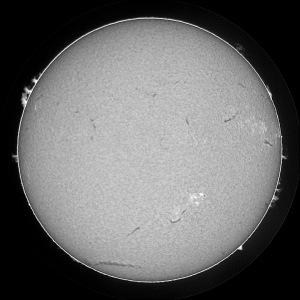
\includegraphics[width=1.0cm]{figures/thumb_input.png}};
  \node[note, below=2pt of img] {photograph};
  \node[st=vizblue] (s1) at (0.4,1.2) {Swin stage 1: 1/4};
  \node[st=vizblue] (s2) at (0.4,0.4) {Swin stage 2: 1/8};
  \node[st=vizblue] (s3) at (0.4,-0.4) {Swin stage 3: 1/16};
  \node[st=vizblue] (s4) at (0.4,-1.2) {Swin stage 4: 1/32};
  \draw[flow] (img.east) -- (s1.west |- 0,0);
  \node[big=vizaqua, text width=2.3cm, minimum height=3.0cm] (pd) at (3.35,0)
       {\textbf{\color{inkprimary}pixel decoder}\\[2pt] 6 layers of multi-scale deformable attention on 1/8, 1/16, 1/32; upsampled and fused to 1/4};
  \foreach \s in {s1,s2,s3,s4} \draw[flow] (\s.east) -- (\s.east -| pd.west);
  \node[big=vizorange, text width=2.55cm, minimum height=3.0cm] (dec) at (6.75,0)
       {\textbf{\color{inkprimary}transformer decoder}\\[2pt] 9 layers; each: masked cross-attention to one scale (1/32, 1/16, 1/8 in turn), self-attention among queries, MLP};
  \node[st=vizorange, text width=2.1cm] (q) at (6.75,2.2) {100 learned object queries};
  \draw[flow] (q) -- (dec);
  \draw[flow] (pd.east |- 0,0.6) -- (dec.west |- 0,0.6);
  \node[st=vizaqua] (F) at (3.35,-2.35) {per-pixel embeddings $\mathbf{F}$ at 1/4};
  \draw[flow] (pd) -- (F);
  \node[st=vizorange, text width=1.8cm] (cls) at (9.6,0.8) {class: filament or no object};
  \node[st=vizorange, text width=1.8cm] (emb) at (9.6,-0.4) {mask embedding $\mathbf{e}_q$};
  \node[st=inkmuted, text width=1.8cm] (mask) at (9.6,-2.35) {mask $\sigmoid(\mathbf{e}_q^{\top}\mathbf{F})$ at 1/4};
  \draw[flow] (dec.east |- cls) -- (cls);
  \draw[flow] (dec.east |- emb) -- (emb);
  \draw[flow] (emb) -- (mask);
  \draw[flow] (F) -- (mask);
  \draw[dashflow] (mask.north west) to[bend left=18] (dec.south east);
  \node[note] at (6.75,-1.93) {each layer's masks restrict\\ the next layer's attention};
\end{tikzpicture}
\caption{Mask2Former as used in this project. The Swin-S backbone produces four feature maps. The
pixel decoder refines the three coarsest with deformable attention and produces per-pixel embeddings
at a quarter of the input resolution. The 100 queries pass through nine decoder layers, each of which
attends only inside the query's current mask, and each query ends with a class and a mask.
\drawnin{book/chapters/ch11\_transformers.tex}}
\label{fig:tr-m2f}
\end{figure}

\subsection{Masked attention}\label{sec:tr-masked}
In MaskFormer, the cross-attention of each query looks at the whole image. Mask2Former restricts it to
the query's own object. Before each decoder layer $\ell$, the query's mask predicted by the previous
layer is thresholded at one half, and cross-attention is forbidden outside it. Let $X_\ell$ denote the
query features after layer $\ell$, let $Q_\ell = W_Q X_{\ell-1}$, and let $K_\ell$ and $V_\ell$ be
computed from the image features at the scale used by layer $\ell$. Then
\begin{equation}
X_\ell = \softmax\!\big(\mathcal{M}_{\ell-1} + Q_\ell K_\ell^{\top}\big)\,V_\ell + X_{\ell-1},
\label{eq:tr-masked}
\end{equation}
where the attention mask is
\begin{equation*}
\mathcal{M}_{\ell-1}(\mathbf{u}) =
\begin{cases} 0 & \text{if } m_q^{\ell-1}(\mathbf{u}) \ge 0.5,\\ -\infty & \text{otherwise.}\end{cases}
\end{equation*}
The entries equal to $-\infty$ receive zero weight after the softmax, just as the \texttt{forbidden}
argument of Listing~\ref{lst:tr-attention} does. If a query's mask is empty, the restriction is lifted
for that query, so that it can search the whole image. As a result, each query refines its object using
features from the object's own neighbourhood, instead of averaging over the whole photograph, and the
model converges much faster than MaskFormer.

\subsection{Deformable attention in the pixel decoder}\label{sec:tr-deform}
The pixel decoder must let every location of three large feature maps exchange information, which
full attention cannot afford. It therefore uses \keyterm{multi-scale deformable
attention}~\citep{deformabledetr}. Instead of attending to every key, each query attends to a small
number of \emph{sampled} points around a reference location, at every scale
(Figure~\ref{fig:tr-deform}). For a query with features $\mathbf{z}_q$ and a normalised reference point
$\hat{\mathbf{p}}_q\in[0,1]^2$, over the feature maps $\mathbf{x}^1,\dots,\mathbf{x}^L$, the output is
\begin{equation}
\operatorname{MSDeformAttn}(\mathbf{z}_q, \hat{\mathbf{p}}_q)
= \sum_{m=1}^{H} W_m \Big[\sum_{l=1}^{L}\sum_{k=1}^{K} A_{mlqk}\,
W'_m\,\mathbf{x}^{l}\big(\phi_l(\hat{\mathbf{p}}_q) + \Delta\mathbf{p}_{mlqk}\big)\Big],
\label{eq:tr-deform}
\end{equation}
where $m$ runs over $H=8$ heads, $l$ over $L=3$ scales and $k$ over $K=4$ sampled points. The function
$\phi_l$ converts the reference point into the pixel coordinates of level $l$. The offsets
$\Delta\mathbf{p}_{mlqk}$ and the weights $A_{mlqk}$ are predicted from $\mathbf{z}_q$ by linear layers,
and the weights are normalised by a softmax over the pairs $(l,k)$. The offsets are fractional, so the
feature map $\mathbf{x}^l(\cdot)$ is read by \keyterm{bilinear interpolation} of its four nearest
feature vectors.

Each query therefore touches only $H\cdot L\cdot K = 96$ sampled points instead of every location, so
the cost is linear in the number of pixels. The offsets are also learned, so the model decides where
to look. In the pixel decoder, every location of the three coarsest maps acts as a query, with
its own position as the reference point, and six such layers are stacked.

\begin{figure}[t]
\centering
\begin{tikzpicture}[
  sp/.style={circle, fill=vizorange, inner sep=0pt, minimum size=4pt},
  rp/.style={draw=inkprimary, line width=0.9pt, cross out, minimum size=5pt, inner sep=0pt}]
  \foreach \sx/\n/\lab in {0/8/{level 1: fine}, 2.9/4/{level 2}, 5.8/2/{level 3: coarse}}{
    \begin{scope}[xshift=\sx cm]
      \pgfmathsetmacro{\gstep}{2.2/\n}
      \fill[vizaqua!10] (0,0) rectangle (2.2,2.2);
      \draw[gridline, line width=0.4pt, step=\gstep cm] (0,0) grid (2.2,2.2);
      \draw[inkmuted, line width=0.6pt] (0,0) rectangle (2.2,2.2);
      \node[rp] at (1.2,1.0) {};
      \node[note] at (1.1,-0.3) {\lab};
    \end{scope}
  }
  \foreach \dx/\dy in {0.35/0.45, -0.4/0.25, 0.15/-0.45, 0.6/-0.1}
    { \node[sp] (p) at (1.2+\dx,1.0+\dy) {}; \draw[->, line width=0.5pt, draw=vizorange!80!black] (1.2,1.0) -- (p); }
  \foreach \dx/\dy in {0.55/0.6, -0.65/0.1, 0.3/-0.6, -0.2/0.75}
    { \node[sp] (p) at (4.1+\dx,1.0+\dy) {}; \draw[->, line width=0.5pt, draw=vizorange!80!black] (4.1,1.0) -- (p); }
  \foreach \dx/\dy in {0.7/0.8, -0.85/-0.3, 0.45/-0.75, -0.5/0.85}
    { \node[sp] (p) at (7.0+\dx,1.0+\dy) {}; \draw[->, line width=0.5pt, draw=vizorange!80!black] (7.0,1.0) -- (p); }
  \node[box=vizorange, text width=2.3cm, font=\sffamily\scriptsize] at (10.3,1.1)
       {weighted sum of the 12 sampled values ($A_{lk}$, softmax over levels and points)};
\end{tikzpicture}
\caption{Multi-scale deformable attention for one head. The same reference point (cross) is located
at every level. The query predicts four fractional offsets per level (dots) and a weight for each,
reads each value by bilinear interpolation, and returns their weighted sum.
\drawnin{book/chapters/ch11\_transformers.tex}}
\label{fig:tr-deform}
\end{figure}

\subsection{Multi-scale queries and deep supervision}\label{sec:tr-deep}
The transformer decoder has nine layers, and they use the scales produced by the pixel decoder in
turn: layer 1 attends to the map at stride 32, layer 2 to the map at stride 16, layer 3 to the map at
stride 8, and the cycle repeats three times. The coarse maps provide context cheaply, and the fine maps
provide detail. Each layer also performs cross-attention \emph{before} self-attention, so that the
queries look at the image before they coordinate with each other, and the initial features of the
queries are learned, whereas MaskFormer sets them to zero.

A prediction, consisting of a class and a mask for every query, is made from the initial queries and
again after each of the nine layers. All ten predictions are matched to the annotations and all ten
are penalised. This is called \keyterm{deep supervision}~\citep{lee2015dsn}: every layer is trained to produce a usable
answer, so the gradients reach the early layers directly.

\subsection{The loss, with point sampling}\label{sec:tr-loss}
For a matched pair of a query and an annotated filament, the loss has three terms: a cross-entropy on
the class, a per-pixel binary cross-entropy between the predicted and annotated masks, and a Dice loss
(Equation~\eqref{eq:par-dice}),
\begin{equation}
\mathcal{L} = \lambda_{\text{cls}}\mathcal{L}_{\text{cls}} + \lambda_{\text{mask}}\mathcal{L}_{\text{BCE}}
+ \lambda_{\text{dice}}\mathcal{L}_{\text{Dice}}, \qquad
(\lambda_{\text{cls}}, \lambda_{\text{mask}}, \lambda_{\text{dice}}) = (2, 5, 5),
\label{eq:tr-loss}
\end{equation}
with the ``no object'' class weighted by 0.1 in the cross-entropy. The mask and Dice terms are summed
over the matched pairs and divided by the number of annotated masks in the batch, and the class term is
normalised by the total class weight. The matching cost of Equation~\eqref{eq:tr-matching} uses the
same three terms.

Evaluating the mask terms at every pixel of a crop of 1024 pixels, for up to 100 queries and ten
predictions, would be very expensive. Mask2Former therefore evaluates them at a sample of $P = 12{,}544$
points per mask, chosen by \keyterm{importance sampling}~\citep{pointrend}. It draws $3P$ points
uniformly at random, keeps the $0.75P$ of them at which the prediction is most uncertain (those whose
logit is closest to zero, which lie along the predicted boundary), and adds $0.25P$ fresh uniformly
drawn points. The annotated mask is read at the same continuous coordinates by bilinear interpolation.
Two consequences of this scheme matter for us. First, the loss concentrates on boundaries, where
Chapter~\ref{ch:post} found most of the error. Second, because the annotated mask is sampled at
fractional positions of a target at the native resolution, the supervision is finer than the model's
output grid at stride 4.

\subsection{The configuration we used}\label{sec:tr-config}
We used version 4.57.6 of the Hugging Face \texttt{transformers} implementation~\citep{wolf2020} with the checkpoint
\texttt{facebook/\allowbreak mask2former-\allowbreak swin-\allowbreak small-\allowbreak coco-\allowbreak instance}.\footnote{Several details in this chapter, such
as the normalisation of the positional embeddings, were read from the source code of this pinned
version rather than from the paper, because the two can differ.} The model has about 69 million
parameters,
100 queries and a hidden size of 256, and we used its loss exactly as shipped. We re-initialised the
classification head for a single class. At most 26 filaments appear in any validation record, and at
most 23 in any training record, so 100 queries are never too few.

\subsection{From queries to scored masks}\label{sec:tr-inference}
At test time every query yields a candidate. Its class probability $p_q$ is the softmax probability of
``filament'' against ``no object''. Its mask logits are enlarged from a quarter of the resolution to
$2048\times2048$ by bilinear interpolation, and thresholded at zero, which corresponds to a probability
of one half. Its score multiplies the class probability by the mean mask probability inside the binary
mask,
\begin{equation}
s_q = p_q \cdot \frac{\sum_{\mathbf{u}} \sigmoid(m_q(\mathbf{u}))\,\mathbf{1}[m_q(\mathbf{u})>0]}
{\sum_{\mathbf{u}} \mathbf{1}[m_q(\mathbf{u})>0]} ,
\label{eq:tr-score}
\end{equation}
where $m_q(\mathbf{u})$ now denotes the upsampled mask logit. The second factor rewards confident
masks: a query that is sure that a filament exists but unsure of its extent receives a lower score.
Listing~\ref{lst:tr-predict} shows our implementation.

\begin{lstlisting}[caption={Candidates from one forward pass. Condensed from
\file{experiments/exp\_139\_mask2former/src/model.py:predict}.},label=lst:tr-predict]
@torch.inference_mode()
def predict(model, gray, device, floor=0.02, min_pixels=40, chunk=8):
    pixels = gpu_pixels(torch.from_numpy(gray)[None], None, device)   # grey -> 3 channels, normalised
    output = model(pixel_values=pixels)
    probability = output.class_queries_logits[0].float().softmax(-1)[:, 0]   # filament vs no object
    logits = output.masks_queries_logits[0]                                  # (100, H/4, W/4)
    keep = torch.nonzero(probability >= floor).flatten()
    candidates = []
    for start in range(0, len(keep), chunk):                                 # bounded memory
        queries = keep[start:start + chunk]
        upsampled = F.interpolate(logits[queries][None].float(), size=gray.shape,
                                  mode="bilinear", align_corners=False)[0]   # to 2048 x 2048
        binary = upsampled > 0
        area = binary.flatten(1).sum(1)
        inside = (upsampled.sigmoid() * binary).flatten(1).sum(1) / area.clamp(min=1)
        scores = probability[queries] * inside       # class probability x mean mask probability
        for j in range(len(queries)):
            if int(area[j]) >= min_pixels:
                candidates.append((float(scores[j]), binary[j].to(torch.uint8).cpu().numpy()))
    return candidates
\end{lstlisting}

The candidates then pass through the same emission rule that we used for every earlier model. We keep
the candidates whose score clears a threshold, paint them in order of decreasing score so that the
masks become disjoint (Section~\ref{sec:masks-paint}), and drop pieces smaller than a minimum area. For
the deployed model, the threshold was 0.85, with no erosion and a minimum area of 100 pixels
(Chapter~\ref{ch:submission}).

\section{Why this architecture suits filaments}\label{sec:tr-why}
Three properties connect Mask2Former to the lessons of the earlier chapters. We argue for each of
them here, and the following chapters measure them.
\begin{enumerate}[leftmargin=*,itemsep=2pt]
\item \textbf{Each filament is predicted once.} The one-to-one matching trains the model to describe
every object once, without a step that suppresses duplicates. The YOLO pipeline needed non-maximum
suppression and, at its best, fusion over eight views, whereas a single view of the Mask2Former beat
every fused YOLO pipeline.
\item \textbf{Each mask is built from the image, for its own object.} A YOLO mask mixes 32 prototypes
that are shared by the whole photograph. A Mask2Former mask comes from a 256-dimensional embedding that
its query computed by attending, through masked attention, to the neighbourhood of its own object.
\item \textbf{The masks lie on a grid of stride 4 in native pixels.} The masks are predicted at a
quarter of the input resolution, so if the input is the native photograph, the mask grid has cells
four native pixels wide. Section~\ref{sec:train-resolution} shows that a perfect mask on this grid
could still reach a mean IoU of 0.914 with the annotations, whereas a grid with cells eight native
pixels wide is limited to 0.771.
\end{enumerate}
The price is memory and engineering effort. The model is large, its attention is irregular, and
training it at the native resolution on thousands of crops required the careful work described in
Chapter~\ref{ch:training}.

\section*{Exercises}
\begin{exercise}{Why divide by $\sqrt{d_k}$?}\label{ex:tr-sqrt}
Let $\mathbf{q},\mathbf{k}\in\R^{d}$ have independent components with mean 0 and variance 1. Show that
$\mathbf{q}^{\top}\mathbf{k}$ has variance $d$. What happens to the softmax of $n$ such scores as $d$
grows, if the scores are not scaled?
\end{exercise}

\begin{exercise}{The cost of windows}
For a crop of $1024\times1024$ pixels, compute the number of tokens at stride 4, and the number of
attention scores per layer with global attention and with windows of $7\times7$ tokens. How much memory
would the global matrix of scores need in 16-bit floating point?
\end{exercise}

\begin{exercise}{The sine embedding across extents}
Using Equation~\eqref{eq:tr-sine}, compute the difference between the embeddings of two pixels 16
native pixels apart, in a crop of 1024 pixels and in a frame of 2048 pixels, for the lowest and the
highest frequencies. Explain why a model trained only on crops sees an unfamiliar pattern of positions
at 2048 pixels.
\end{exercise}

\begin{exercise}{Greedy versus Hungarian}
Construct a $3\times3$ cost matrix on which greedy matching costs more than three times as much as the
optimal matching. Can the greedy matching ever be worse than the optimal one when every row and every
column has a single, clearly cheapest entry?
\end{exercise}

\begin{exercise}{Point sampling}
Implement importance sampling for one predicted mask: draw $3P$ uniform points, keep the $0.75P$ most
uncertain ones, and add $0.25P$ uniform points. On a real filament mask and a slightly shifted
prediction of it, compare the Dice loss computed on the sampled points with the Dice loss computed on
all pixels, for $P$ between 100 and 12,544.
\end{exercise}
